\documentclass[a4paper,11pt,titlepage]{article}

\usepackage[breaklinks=true]{hyperref}

\usepackage{pdflscape}

% encoding
\usepackage[utf8]{inputenc}
\usepackage[T1]{fontenc}

%Collaboration management
\usepackage[draft,english]{fixme}
%read-me: http://mirrors.dotsrc.org/ctan/macros/latex/contrib/fixme/fixme.pdf

% layout
\bibliographystyle{ieeetr}

\usepackage[margin=3cm]{geometry}
\usepackage{textcomp}

% appearance
\usepackage{graphicx} 
\usepackage{color}

% math extensions
\usepackage{amsmath}
\usepackage{amssymb}
\usepackage{amsthm}
\usepackage{listings}

\lstset{%
  frame=trBL,
  frameround=fttt,
  basicstyle=\footnotesize\tt,
  keywordstyle=\bf,
  language = C,
  tabsize=2
}
\newcommand{\for}{\text{ for }}
\newcommand{\then}{\rightarrow}
\newcommand{\id}[1]{\ensuremath{\mathop{\mathit{#1}}\nolimits}}

% header and footer
\usepackage{fancyhdr}

\definecolor{qstgray}{gray}{0.9}
\makeatletter
\newenvironment{qst}{
  \begin{lrbox}{\@tempboxa}
    \begin{minipage}{\columnwidth}
      \footnotesize \slshape
    }
    {
    \end{minipage}
  \end{lrbox}
  \colorbox{qstgray}{\usebox{\@tempboxa}}
}
\makeatother

\fancypagestyle{fncy}{
  \lhead{\thecourse}
  \chead{\today}
  \rhead{Handin 2}
  \lfoot{}
  \cfoot{}
  \rfoot{\thepage}
  \renewcommand{\headrulewidth}{0.5pt}
  \renewcommand{\footrulewidth}{0.5pt}
}

\setcounter{secnumdepth}{2}
\setcounter{tocdepth}{2}

%\pagestyle{fncy} can't be used with progress 

% title
\title{\thecourse \\ \thetitle} 
\date{\today} 
\author{%
  \begin{tabular}{ll}
    Frederik Mogensen & 20080923\\
    Allan Stisen & 20083311\\
    Lasse Højgaard & 20080848
  \end{tabular}
}



\newcommand{\thecourse}{Wireless Sensor Networks}
\newcommand{\thetitle}{Mini-project 3 - Temperature sensing} 
\newcommand{\subsubsubsection}[1]{\underline{#1}\newline}

\begin{document}

\maketitle
\newpage

\tableofcontents
\newpage
\section{Project Description}
In the following project we've made a sensor network which can measure the temperature periodically. The sensor motes will transmit their results (different strategies will be covered and discussed in the extension part) to the sink which indicates the temperature by either a blue ($\leq 15^{\circ} C $) or a red $>15^{\circ} C$.

To make sure that the sink has received the packages the sink will send an ACK to the sensing mote, if the sink receives the sensing data correctly. After receiving an ACK the sensing mote goes to sleep, if not it receives an ACK it will try to retransmit $N$ times.

\section{Project implementations}
The project implementation is divided in several sections, where each section is described. First we've got an overall description of the project which we've implemented.

\subsection{Overall description}
\begin{figure}[htbp]
   \centering
   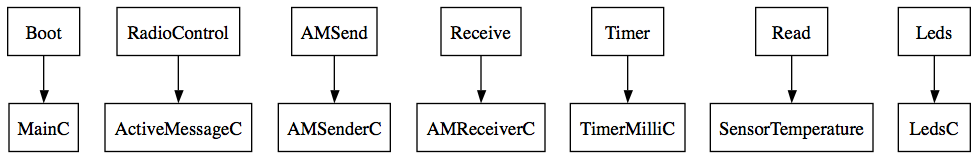
\includegraphics[width=17cm]{SWgraph.png} 
   \caption{An overall illustration of the project implmented}
   \label{fig:overalloverview}
\end{figure}

\subsection{Temperature measuring}
Here we'll explain how and where we convert the digital readout from the temperature sensor to actual degress.
The conversion given a digital readout ($SO_{T}$) to a temperature value is given at the following formula\cite{temperature}:
\begin{align*}
	T &= d_{1} + d_{2} \cdot SO_{T}
\end{align*}
where the coefficients is defined in Tabel ~\ref{table:temperature}
\begin{table}[ht]
\centering
\begin{tabular}{ | l | c | r | }
	\hline
	VDD & $d_{1} \ ^{\circ}  C$ & $d_{1} \ ^{\circ}  F$ \\
	\hline \hline
	5V & -40.1 & -40.2 \\
	\hline
	4V & -39.8 & -39.6 \\
	\hline
	3.5V & -39.7 & -39.5 \\
	\hline
	3V & -39.6 & -39.3 \\
	\hline
	2.5V & -39.4 & -38.9 \\
	\hline
\end{tabular}
\begin{tabular}{ | l | c | r | }
	\hline
	$SO_{T}$ & $d_{2}  \ ^{\circ}C$ & $d_{2} \ ^{\circ} F$ \\
	\hline \hline
	14 bit & 0.01 & 0.018 \\
	\hline
	12 bit & 0.04 & 0.072\\
	\hline
\end{tabular}
\caption{Temperature conversion coefficients}
\label{table:temperature}
\end{table}
The conversion from a digital readout is being done in the event readDone. We've made two compile time constants, $CONVERSION_{D1}$, and $CONVERSION_{D2}$.
\begin{lstlisting}
CONVERSION_D1 = 3960, /* VDD = 3V */
CONVERSION_D2 = 1 /* 14 bits */
...
event void Read.readDone(error_t result, uint16_t data) {
	float tempC;
	if (result != SUCCESS){
		data = 0xffff;
		report_problem();
	}
	  // conversion
	  tempC = ( (-CONVERSION_D1) + (CONVERSION_D2 * data) ) ;
    local.readings[reading++] = tempC;
}
\end{lstlisting}


\subsection{Network communication}

\begin{lstlisting}
message_t* receive(message_t *msg, void *payload, uint8_t len) {
		message_t *ret = msg;
		int avg = 0, i = 0;

		if (len == sizeof(temperature_t)) {
			temperature_t* tmpptr = (temperature_t*)payload;
			printf("\n---------------------------\n");
			for (i = 0; i < NREADINGS ; i++) {
				avg = avg + tmpptr->readings[i];
				printf("%d %d \n", tmpptr->count*10 + i, tmpptr->readings[i]);
			}
			avg = avg / NREADINGS;
			printf("average: %d\n", avg);
			printfflush();
			if (avg <= 2800) {
				call Leds.led1Off();
				call Leds.led0On();
			} else {
				call Leds.led0Off();
				call Leds.led1On();
			}
		}
\end{lstlisting}

\section{Extensions of Project}
\begin{description}
\item[Multiple motes] If there are multiple sensing motes, they send their sensing data to the sink.
\item[Plotting] Plot temperature vs. time (offline /online)
\item[Temperature average] The sink averages the temperature from the sensors.
\item[Temperature average sensor] The sensor motes averages $n$ temperatures before sending to the sink to improve energy efficiency of the application.
\item[Temperature average improved] Motes averages temperature sends number of recorded temperatures which indicates what weight the sink should use to make a correct average.

\end{description}

\section{Energy efficiency}
\section{Project results}
put various graphs here


\newpage
\bibliography{references}
\end{document}
